\chapter{Evaluation}
\label{chap:Evaluation}

In this chapter, we will go through our experimental hypothesis, testing scenarios, experiments conducted on two sample 
stereo matching algorithms, SGBM and ADCensus mentioned in chapter \ref{chap:Introduction}, and the results with our
proposed evlaution system to assess the benefits of using our evaluation model for a 3D AR application over the general-purpose evluation models; 
Middlebury and Kitti Evaluation stereo evaluation.

\section{Stereo Dataset}
It should be noted that the stereo dataset we have used to conduct the experiments on stereo matching algorithms in our system,
are selected from Kitti Stereo Dataset.
In contrary to Middlebury dataset, Kitti Stereo Project provides stereo images and ground truth disparity maps
that are taken from outdoor scenes under real circumstances. This property of sample images makes them more appropriate 
for evaluating the performance of the stereo algorithms in practical AR application, thus better meeting our objectives in this research.
We have selected 52 samples image pairs among Kitti Stereo dataset based on different photometric and visual properties that are important
in stereo vision and an AR application. Some 
of these properties are listed as follows:
\begin{itemize}
\item light and shading; i.e. selecting scenes containing bright, dim, and dark regions
\item Various depth ranges; i.e. selecting scenes that contains near field, medium field and far field objects  
\item Depth discontinuity and Occlusion
\item Well textured and textureless regions
\end{itemize}


\section{Methodology}

Before going through the explanation of the experiments conducted to assess our evaluation model, we phrase our main research question in this
study once more here to better justify our hypotheses and the selected experiments. 
As mentioned earlier in chapter \ref{chap:Introduction}, our main objective is to investigate whether using 
stereo matching techniques to generate the depth map of the 
surrounding environment in an AR application can meet the requirements of a practical AR system. 
Therefore, our experiments focus 
on assessing those aspects of our evaluation model that assist to better answer this question.
As a result, our first attempt towards evaluating our model is to investigate and demonstrate whether the results of the evaluation process 
are properly measured and presented based on the important factors in the augmented reality framework.
After confirming the aforementioned property, which is the key property of our model, we investigate the effect of our proposed masking 
procedure on the evaluation process. Moreover, we present how the methods can be evaluated for use in real-time applications. 

We also explain how the evaluation and comparison of the methods is done in our model by conducting some
experiments on sample stereo matching algorithms based on the specific factors
which have been the focus of this study.

\subsection{Hypotheses}

We have defined a set of hypotheses to evaluate our proposed design. These hypotheses are as follows:

\begin{itemize}
\item \textbf{Hypothesis 1}: \emph{Our model evaluates and demonstrates the stereo matching algorithm performance in the framework of augmented reality} 
Unlike Middlebury and Kitti benchmarks which can be counted as general-purpose evaluation models, our system can particularly evaluate the algorithms in the framework of an 
augmented reality application to facilitate the process of determining
the proper method for using in an AR system for real-time generation of depth of the surrounding environment.

\item \textbf{Hypothesis 2:} \emph{Observing, evaluating and refining the areas near the depth edges in an image is more important in an AR application}
Salient edges, which can also represent the object boundaries and occlusion, are one of the 
most important depth cues that helps the observer to better perceive the depth of different objects in the scene. In other words, the areas near the edges corresponding to depth discontinuities
in a scene are more important to human visual system for perception of depth in an AR application and therefore, the disparity 
errors in these regions can be detected easier by HVS. Therefore, we argue that in our model, the evaluation of the disparity results in these regions can be of great value 
to an AR application.

\item \textbf{Hypothesis 3:} \emph{Our system is better than other evaluation models in terms of assessing the performance of the algorithm for real-time applications}  
Other evaluation models, Kitti and Middlebury, do not evaluateand report on the performance of the algorithms
with respect to real-time application requirements. On the other hand, our system is capable of examining and evaluating the algorithms 
based on their execution time and therefore, can report on
their suitability for real-time AR applications.

\end{itemize}

The experiments designed to validate these hypotheses are explained in the following section.

\section{Experimental Environment and Settings}
Experiments were carried out on a Linux machine with Core(TM) i7 3.20GHz CPU. 
The set of parameters used at different steps of the evaluation process are presented in the following sections.
It should be noted that the parameters were kept constant for all the images and most of the experiments. 
However, it will be explicitly mentioned if a parameter has been used with a different value in any of the experiments due to specific reasons.

\subsection{Dilation and Canny settings}
We have used Dilation operation for expanding the detected edge regions in the masking process. The extent of this expansion
is determined by the number of iterations for dilating the masked areas. Table \ref{tab:candilparam} presenet the parameters used in Dilation
and Canny edge detection. However, the \textit{minimum threshold} in Canny detection was tuned and selected seperately for each image, 
since the threshold may differ depending on the scene.

\begin{minipage}{\linewidth}
\begin{center}
\captionof{table}{Masking Parameters}
\label{tab:candilparam}
\begin{tabular}{ |c|c| }
\hline
\textbf{Params} & \textbf{Value} \\ \hline
dilation\_itr & 10 \\  \hline
Canny\_ratio & 3 \\ \hline
\end{tabular}
\end{center}
\end{minipage} \newline

It should be noted that, since the ground truth disparity available for Kitti stereo data has been generated by a 3D laser scanner,
it is a point cloud map of discrete disparity values. This nature of the disparity maps appeared to be troublesome in the masking process as all the gaps
between the disparity points were causing them to be counted as disconnected edges. Therefore, to correctly detect the 
depth edges in the image, first we needed to fill in the gaps and obtain a smoothed ground truth disparity. We used Dilation for this pupose as well but with different number
of iterations for each image depending on the scene and the original ground truth disparity map.


\subsection{Stereo algorithms settings}
The parameters for each algorithm that were used in our experiments to generate disparity
maps were also kept constant over all the images in the dataset. These parameters are presented in tables \ref{tab:sgbmparams} and \ref{tab:adcparams} 
for SGBM and ADCensus respectively. \newline

\begin{minipage}{0.8\linewidth}
\begin{center}
\captionof{table}{SGBM Parameters}
\label{tab:sgbmparams}
\begin{tabular}{ |c|c|c| }
\hline
SADWindowSize & disp12MaxDiff & uniquenessRatio\\  \hline
9 & 2 & 10 \\ \hline
P2 & speckleWindowSize & speckleRange \\ \hline
3*SADWindowSize & 100 & 2  \\ \hline
\end{tabular}
\end{center}
\end{minipage} \newline \newline

Others parameters that have not been mentioned in the table were considered with their default values. \newline

\begin{minipage}{0.8\linewidth}
\begin{center}
\captionof{table}{ADCensus Parameters}
\label{tab:adcparams}
\begin{tabular}{|c|c|c|c|c|c|}
\hline
$\lambda_{AD}$ & $\lambda_{Census}$ & $L_{1}$ & $L_{2}$ & $\tau_{1}$ & $\tau_{2}$ \\  \hline
10 & 30 & 34 & 17 & 20 & 6  \\ \hline
$\pi_{1}$ & $\pi_{2}$ & $\tau_{SO}$ & $\tau_{S}$ & $\tau_{H}$ & \\  \hline
1.0 & 3.0 & 15 & 20 & 0.4 &  \\ \hline
\end{tabular}
\end{center}
\end{minipage} \newline

The minimum and maximum disparity were also kept constant for each image between the algorithms; however, the maximum disparity differ for each image pair as the scenes are different
and objects are located at different depth ranges.
The minimum disparity was set to $0$ in both algorithms. Maximum disparity was set based on the maximum disparity value in the ground truth corresponding to each
image pair. The only restriction here was to choose the closest value greater than or equal to the maximum disparity of ground turth that is a multiplication of 16. This restriction
is implied by the implementation of SGBM algorithm.

\subsection{Evaluation Params}
In our evaluation model, due to the large number of output data which grows as more images are added to the input selection, 
plots are generated by taking an average of the whole generated outputs. This average results from two steps; first, getting an average of the relative depth error over specific
depth ranges for each image and then getting the average of the values from the previous step over all of the images. This operation finally results in a single plot
that demonstrate the average error of relative depth within specific distance.
The averaging opertion at this step are implemented by building histogram over the data. The number of bins was set to 100 and the width of each bin was set to 0.5; 
i.e. averaging results over half a meter. Therefore the maximum distance over which the output is being examined is 50m.

\subsection{Assumption}
\textbf{Talk about camera quality and display resolution}

\subsection{Experiments}
In this section we discuss the experiments conducted to evaluate the system and investigate the validity of the hypotheses.

\subsection{Evaluation results in augmented reality framework}

In this experiment, the disparity maps 
were generated for fifty-two image pairs with both SGBM and ADCensus. 
After generating the corresponding disparity maps for all the images, 
the evaluation process was conducted on each map seperately and the average disparity errors, over the distance range of half a meter,
for each image was generated.

Sample plots corresponding to one of the stereo pairs, shown in figure \ref{fig:img5},
over the masked areas are displayed in figures \ref{fig:imgmsk} and \ref{fig:imgfull}, respectively.

\begin{figure}[h!]
\centering
\subcaptionbox{Left image}
[.5\linewidth]{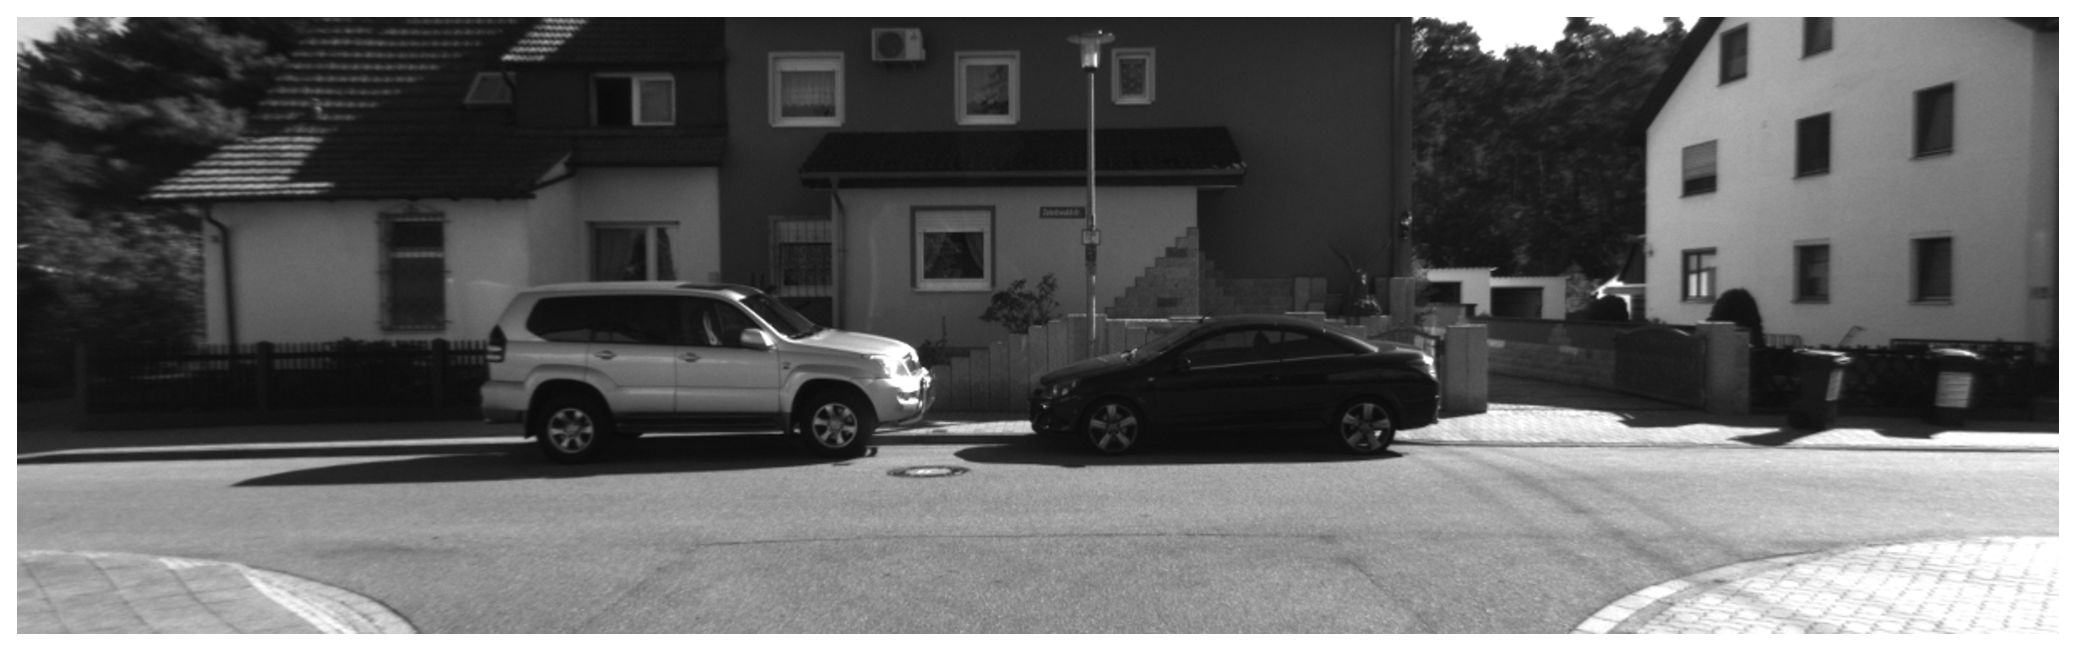
\includegraphics[scale=0.21]{000005L}}%
\subcaptionbox{Right image}
[.5\linewidth]{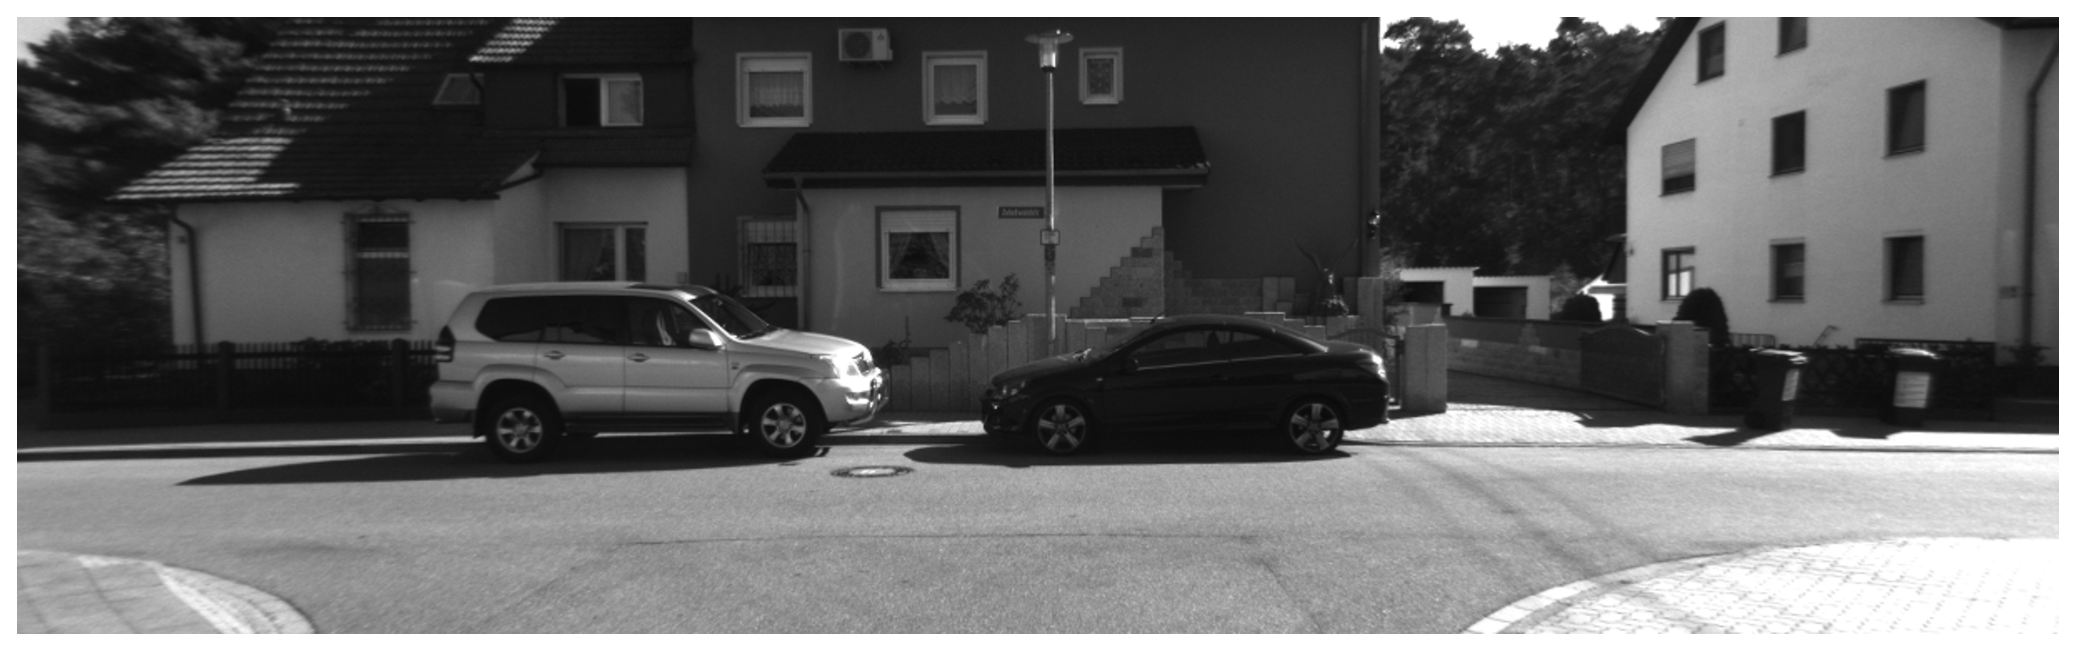
\includegraphics[scale=0.21]{000005R}}%
\caption{Sample stereo image from Kitti}
\label{fig:img5}
\end{figure}

\begin{figure}[H]
\centering
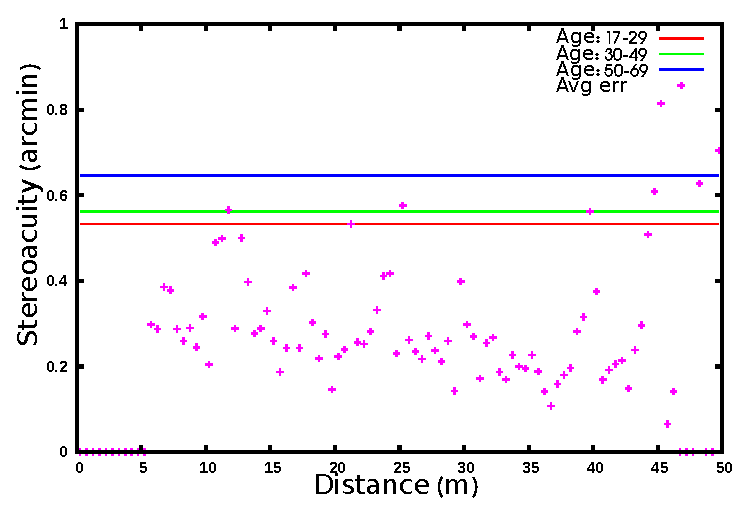
\includegraphics[scale=0.8]{sgbmimg5pix3msk}
\caption{Average disparity error over distance by SGBM}
\label{fig:imgmsk}
\end{figure} 

\begin{figure}[H]
\centering
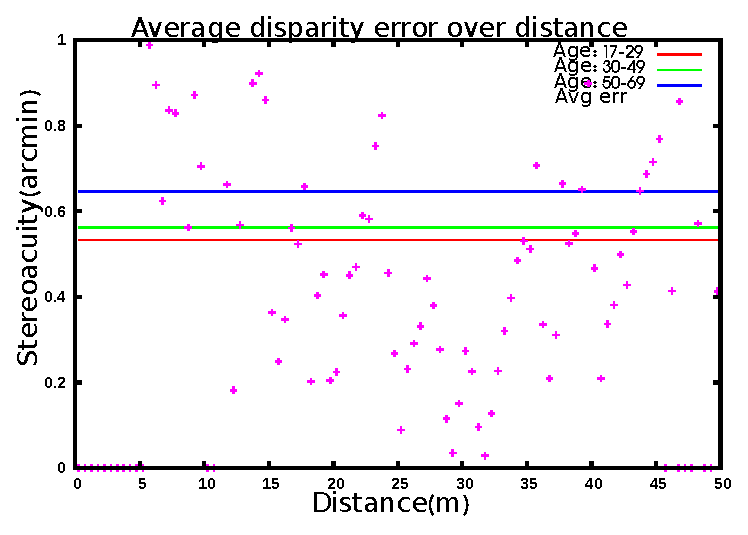
\includegraphics[scale=0.8]{adcimg5pix3msk}
\caption{Average disparity error over distance by ADCensus}
\label{fig:imgfull}
\end{figure}

\noindent
The corresponding mask, figure \ref{fig:imgmsk}; masked ground truth, figure \ref{fig:imggt}; and
the masked disparity images generated by SGBM and ADCensus, figure \ref{fig:5mdispsgb} and \ref{fig:5mdispadc} 
are shown below.

\begin{figure}[H]
\centering

\includegraphics[scale=0.35]{5msk}
\caption{The mask of depth edges and their surrounding regions}
\label{fig:imgmsk}
\end{figure} 

\begin{figure}[H]
\centering

\includegraphics[scale=0.35]{5gt}
\caption{Masked ground truth}
\label{fig:imgmsk}
\end{figure} 

\begin{figure}[H]
\centering

\includegraphics[scale=0.35]{5mdispsgb}
\caption{Masked disparity by SGBM}
\label{fig:imgmsk}
\end{figure} 

\begin{figure}[H]
\centering

\includegraphics[scale=0.35]{5mdispadc}
\caption{Masked disparity by ADCensus}
\label{fig:imgmsk}
\end{figure} 

\noindent
However, due to the large amount of data and in order to obtain a better overview of 
the system behavior, the average of all the results 
was taken for each algorithm.
Final plots, after estimating the average error over all the images, over the masked regions
are shown in figures \ref{fig:mskmapsgbm} and \ref{fig:mskmapadc} by both SGBM and ADCensus, respectively.

\begin{figure}[H]
\centering
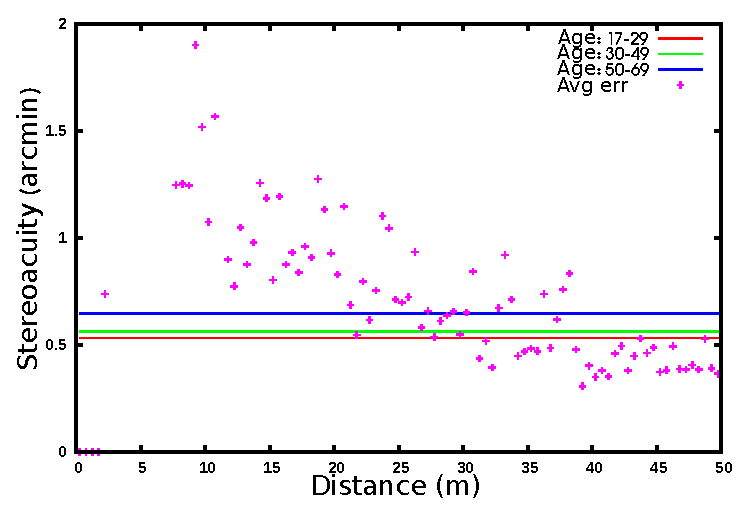
\includegraphics[scale=0.8]{sgbmmsk1000}
\caption{Average disparity error over all the images by SGBM}
\label{fig:mskmapsgbm}
\end{figure} 

\begin{figure}[H]
\centering
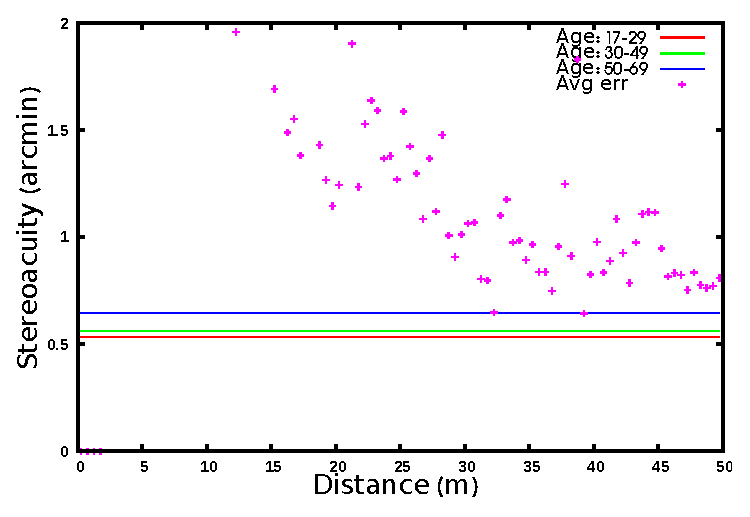
\includegraphics[scale=0.8]{adcenmsk1000}
\caption{Average disparity error over all the images by ADCensus}
\label{fig:mskmapadc}
\end{figure} 

As it can be seen, the average results displayed in the previous plots, contain very sparse points and 
do not demonstrate any consistent pattern. When we investigated the cause of this large variation, we found that in
both algorithms there are some disparity values which have large difference with ground truth disparity and yet have not been invalidated by the
algorithm. However, we assume that these type of outliers can be easily filtered out by applying post processing steps and even if 
not, they will most probably be culled out by the 3D render in AR system in the end. Therefore, we decided to add another filtering condition to our 
evaluation module. In this condition, these types of outliers are first filtered out from the set of examined disparities by being compared
to a threshold value, e.g. 3px, and then the rest of the
evaluation procedure takes place, which is comparing the disparity error to the standard stereoacuities and printing out the results. 
It should be noted that in our design, this \textit{threshold} has been defined as one of the paramateres which can be set 
when running the evaluation process, thus giving the ability of tuning it to any proper value.
This additional condition had a significant impact on the evaluation results. 
In fact, a consistent pattern was observed after filtering out these outliers in the final plots. The results are displayed in
figures \ref{fig:mskmapsgbm} and \ref{fig:mskmapadc}.

\begin{figure}[H]
\centering
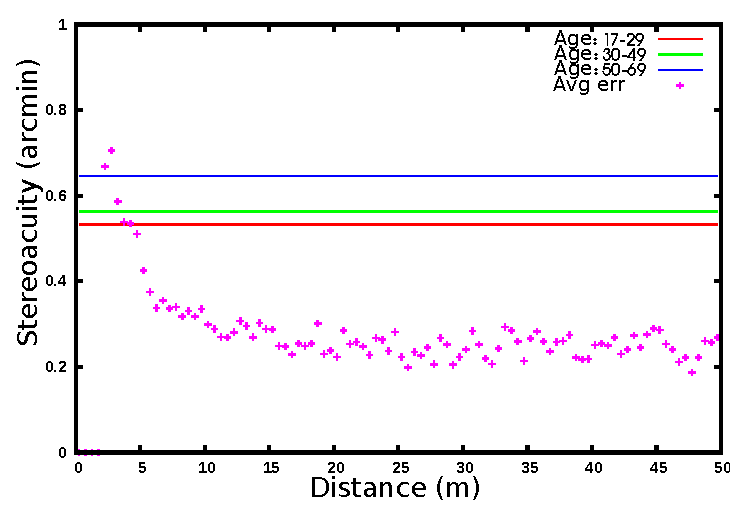
\includegraphics[scale=0.8]{sgbmmsk3}
\caption{Average disparity error over all the images by SGBM}
\label{fig:mskmapsgbm}
\end{figure} 

\begin{figure}[H]
\centering
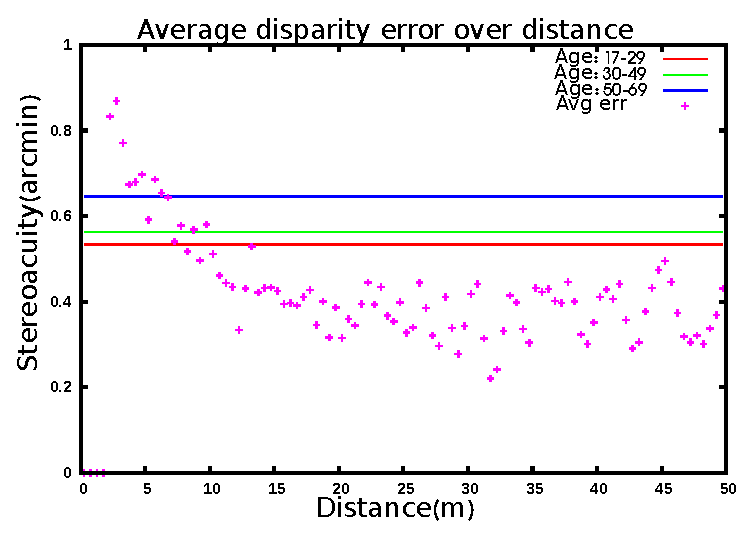
\includegraphics[scale=0.8]{adcenmsk3}
\caption{Average disparity error over all the images by ADCensus}
\label{fig:mskmapadc}
\end{figure} 

In these plots, a cross point below a stereoacuity threshold (straight lines) implies that the average error in the disparity values found by the stereo matching 
algorithm is negligible as the human visual system will not be able to distinguish the difference. 
However, a value more than a threshold indicates that
the error cannot be neglected and should be resolved to achieve a better alignment between the virtual and the 
real world in the AR application of interest.
The zero values in the plots imply that either there has been no object within that range or the disparity value estimated by the algorithm
is equal to the ground truth disparity; however, since the average of the results has been taken over all the images, it is more likely that 
the zero values indicate no object within that range.

As it can be seen in the results, SGBM is performing better in finding more accurate corresponding matches 
compared to ADCensus, as most of the error points fall below the standard stereoacuity lines. Moreover, the plots show that in both methods 
the significant amount of error
corresponds to the near field objects, within the first 5 meters. This range of the depth field can be considerably important in some applications,
such as the ones involving certain manipulative tasks.

\subsection{Depth edges and their surrounding area}
In order to examine the effect of evaluating only certain regions of disparity image; i.e. the depth edges and their surroundings, 
over the whole disparity image, we estimated the average error over the masked areas as well as the full disparity map. 
Results of SGBM are shown below; figure \ref{fig:sgbmfull3} and \ref{fig:sgbmmsk3}

\begin{figure}[H]
\centering
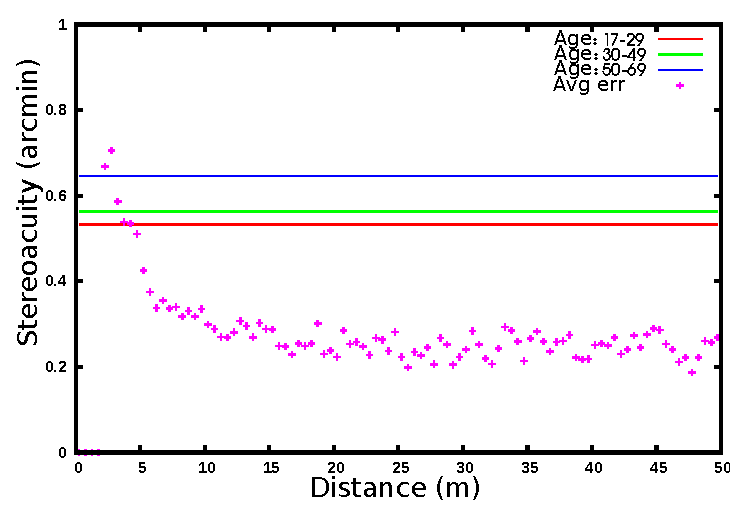
\includegraphics[scale=0.8]{sgbmmsk3}
\caption{Average disparity error over masked areas by SGBM}
\label{fig:sgbmmsk3}
\end{figure} 

\begin{figure}[H]
\centering
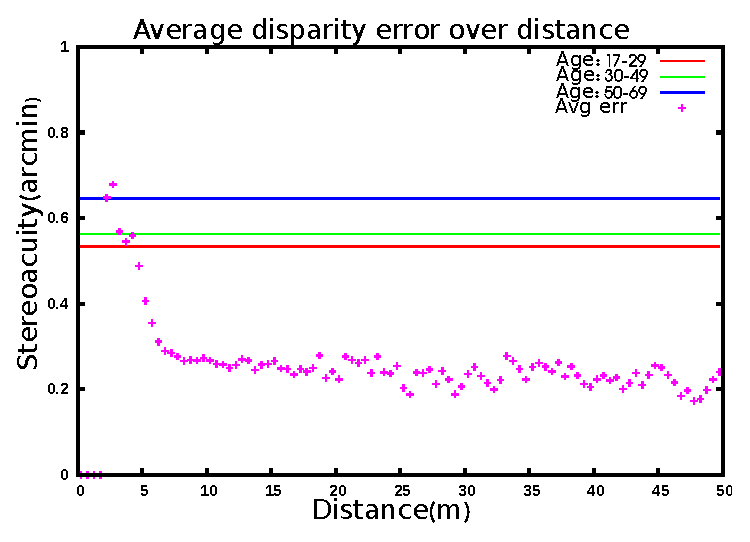
\includegraphics[scale=0.8]{sgbmfull3}
\caption{Average disparity error over all the regions by SGBM}
\label{fig:sgbmfull3}
\end{figure} 



